\section{Naturaleza de los objetivos de aprendizaje}
Un primer conjunto de objetivos de aprendizaje fue propuesto por \cite{Bloom56Taxonomy}. 
Una peque�a variaci�n de la taxonom�a de Bloom es resumida a continuaci�n con algunas 
peque�as adaptaciones al contexto de la computaci�n (utilizando t�rminos como implementar o ejecutar).

En esta discusi�n se siguen los lineamientos de \cite{Anderson2001Bloom}. 
Tipicamente, un objetivo de aprendizaje contiene un verbo y un pronombre:
El verbo describe el proceso cognitivo que se busca. Luego se incluyen los 
elementos de la taxonom�a de Bloom y de esa forma verbos como 
recordar, recordar, entender, analizar, dise�arson altamente relevantes.

Los pronombres describen el conocimiento que se espera que un estudiante adquiera. Luego el conocimiento 
propiamente dicho es categorizado en varias formas en un espectro que va de lo concreto a lo abstracto.

\begin{center}
\begin{table}[h!]
\begin{tabularx}{\textwidth}{|l|l|X|}\hline
\textbf{Nivel} & \textbf{Categor�a}      & \textbf{Proceso Cognitivo} \\ \hline
1.     & Recordar 	& reconocimiento, recordar, describir, declarar (\textit{stating}) \\ \hline
2.     & Entender 	& interpretar, ejemplificar, clasificar, inferir, comparar, explicar, parafrasear, resumir \\ \hline
3.     & Aplicar        & ejecutar (i.e. llevar adelante), implementar (i.e. usar), computar, manipular, resolver \\ \hline
4.     & Analizar      	& diferenciar, organizar, atribuir, discriminar, distinguir, sub-dividir \\ \hline 
5.     & Evaluar     	& verificar, criticar, evaluar (\textit{assess}), comparar, contrastar \\ \hline
6.     & Crear       	& generar, planear, producir, innovar, divisar, dise�ar, organizar \\ \hline
\end{tabularx}
\label{tab:BloomTaxonomy}
\caption{Taxonom�a de Bloom}
\end{table}
\end{center}

Los objetivos del programa tienden a ser asociados con los niveles altos de esta taxonom�a. Asi mismo, 
los objetivos instructivos tienden a ser asociados con los niveles bajos de la misma.

\begin{figure}[h!]
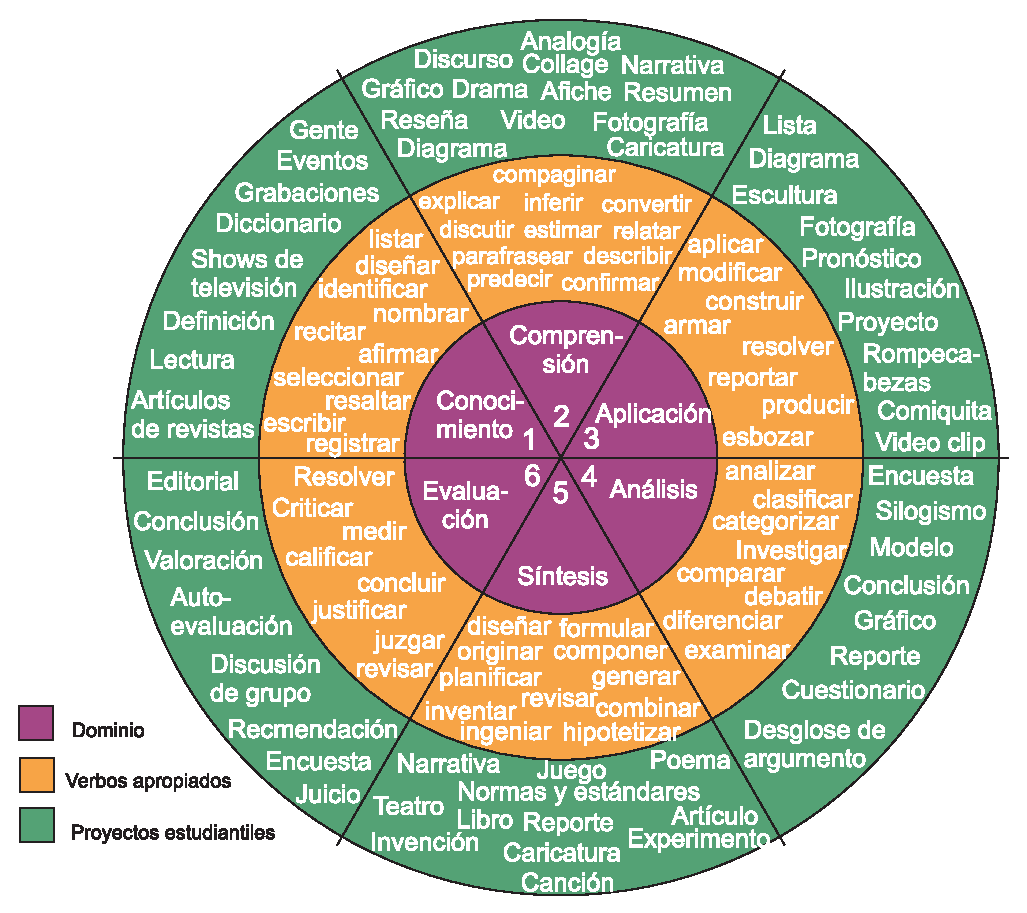
\includegraphics[height=12cm]{\OutputFigDir/Bloom}
\label{fig:BloomTaxonomy}
\caption{Taxonom�a de Bloom}
\end{figure} 
